\section{有序索引}

\subsection{基本概念}

1.在有序索引中,索引条目按搜索键值排序存储,例如图书馆中的作者目录。

2.顺序排序文件:文件(数据文件)中的记录按搜索键排序。

3.主索引:一种索引,其搜索键等于创建该索引的顺序排序数据文件的搜索键(与对应的数据文件本身的排列顺序相同的索引称为主索引)。
也称为聚集索引,主索引的搜索键通常是但并非一定是主码。

以下是一个例子:假设有一张学生信息表\texttt{Student},其定义为:
\begin{lstlisting}[style=sqlstyle]
CREATE TABLE Student (
    StuID CHAR(10) PRIMARY KEY,
    Name VARCHAR(50),
    Major VARCHAR(30),
    Grade INT
);    
\end{lstlisting}

其中\texttt{StuID}是表的主码,且在逻辑上是唯一的。但在物理存储层面,我们并不一定要按照主码来排序。比如为了经常按学生姓名检索,我们可以让数据文件按\texttt{Name}排序。

4.非顺序文件没有主索引,但关系可以有主码。索引顺序文件:带有主索引的顺序有序文件。

5.辅助索引:一种索引,其搜索键指定的顺序与文件的顺序不同。

\subsection{稠密索引文件}

稠密索引:文件中每个搜索键值都有对应的索引项。

例如,教师关系的ID属性上的索引:

\begin{figure}[H]
    \centering
    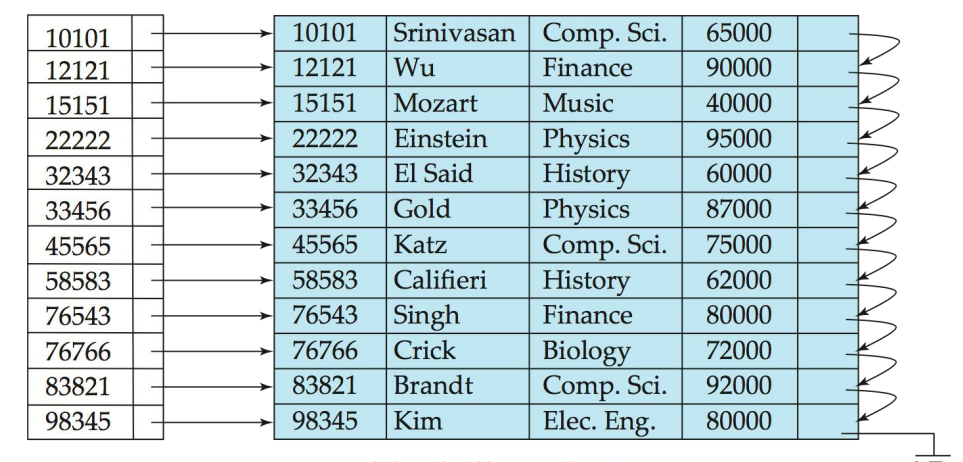
\includegraphics[width=0.9\linewidth]{image1.png}
    \caption{例1}
    \label{}
\end{figure}

基于dept\_name的密集索引,教师文件按depy\_name排序:

\begin{figure}[H]
    \centering
    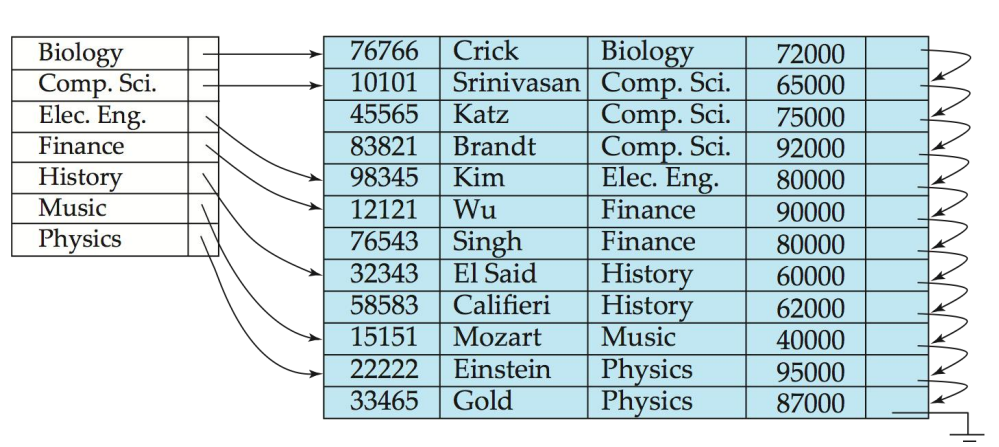
\includegraphics[width=0.9\linewidth]{image2.png}
    \caption{例2}
    \label{}
\end{figure}

\subsection{稀疏索引文件}

稀疏索引:仅包含部分搜索键值的索引项(通常,一个数据块对应一个索引项,一个块包含多个有序的数据记录)。仅适用于数据文件记录按搜索键值顺序排列的情况。

要查找搜索键值为K的记录:

\begin{itemize}
    \item 步骤1:找到搜索键值最大为<K的索引记录
    \item 步骤2:从索引项所指向的记录开始顺序搜索文件
\end{itemize}

\begin{figure}[H]
    \centering
    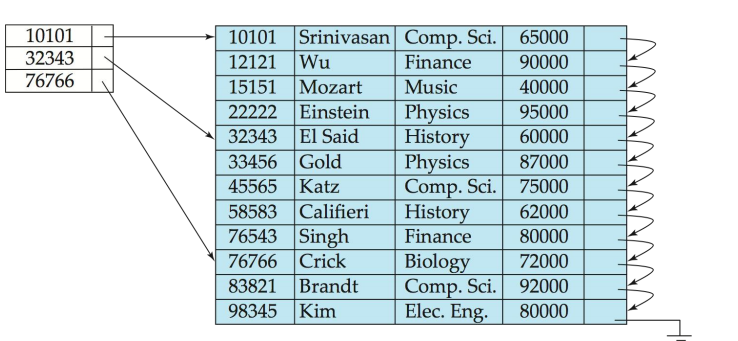
\includegraphics[width=0.9\linewidth]{image3.png}
    \caption{例}
    \label{}
\end{figure}

与密集索引相比:插入和删除操作占用的空间更少,维护开销更低;通常在定位记录方面比密集索引慢。

不错的权衡:为文件中的每个块设置一个索引项的稀疏索引,对应于块中的最小搜索键值(一个块中通常包含多个数据记录,每块中最小的搜索键值放到索引项中)。

稀疏索引只能用于顺序文件,而密集索引可用于顺序和非顺序文件,如构成索引无序文件。

\subsection{二级索引}

通常,人们希望找到某个字段值满足特定条件的所有记录,而该字段并非主索引的搜索键。(实际应用中常有多种属性作为查询条件)

示例:在按账号顺序存储的账户数据库中,我们可能希望找到具有指定余额或余额范围的所有账户。

\begin{figure}[H]
    \centering
    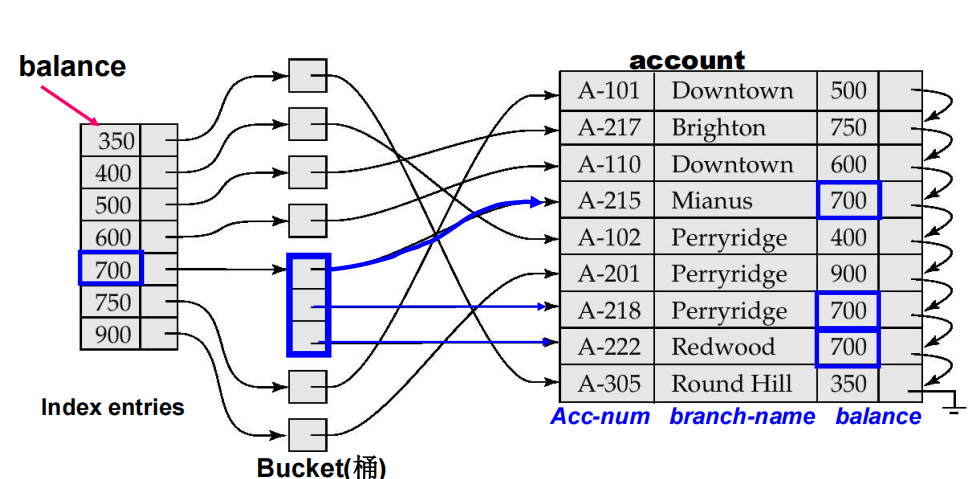
\includegraphics[width=0.9\linewidth]{image4.png}
    \caption{例}
    \label{}
\end{figure}

我们可以为每个搜索键值创建一个二级索引记录;索引记录指向一个桶,该桶包含指向所有具有该特定搜索键值的实际记录的指针。

(辅助索引不能使用稀疏索引,每条记录都必须有指针指向。但search key常存在重复项---如700,而index entry不能有重复,否则查找算法复杂化,为此,使用bucket结构)

\subsection{多级索引}

如果主索引太大而无法装入内容,访问成本会很高。

\noindent例如:1,000,000条记录/每块10条记录=100,000块=100,000个索引项(稀疏索引)/每块100项=1000块(稀疏索引文件的大小)
二分查找:$[\log_2(1000)]=9$次块读取,$10*15ms=150ms$

为减少对索引记录的磁盘访问次数,将保存在磁盘上的主索引视为顺序文件,并在其上构建稀疏索引。(把内层索引文件看作顺序数据文件一样,在其上建立外层的稀疏索引)
\begin{itemize}
    \item 外层索引---主索引的稀疏索引
    \item 内部索引---住索引文件
\end{itemize}

如果即使外部索引也不太大而无法装入主内存,则可以创建另一级别的索引,以此类推(可以推广到任意多层索引)

对文件进行插入或删除操作时,必须更新所有级别的索引。

\subsection{索引更新:删除}

\noindent步骤1:系统在数据文件中找到该记录,然后删除

\noindent步骤2:更新索引文件:(针对单层索引删除)

情况1:密集索引。

如果被删除的记录是具有其特定搜索键值的唯一记录,则从索引文件中删除相应的索引条目(单记录,几搜索键具有唯一性),否则,(多条记录
,即搜索键不具有唯一性)如果有多个指针指向具有相同搜索键值的所有记录,则从索引条目中删除指向已删除记录的指针(对应辅助索引的情况),
否则,(对应主索引)如果被删除的记录是第一个被指向的记录,则将指针更改为指向下一条记录,否则,无需对索引条目进行任何操作。

情况2:稀疏索引。

如果已删除记录的搜索键值未出现在索引中,则无需对索引进行任何操作。否则,如果索引文件中存在该搜索键的索引条目,则通过用数据文件中(按搜索键顺序)的
下一个搜索键值替换该条目来删除它。如果下一个搜索键值已经有索引条目,则直接删除该索引条目,而不是进行替换。

对于多级索引:由底层逐级向上扩展,每一层的处理过程与上述单层索引情况下类似。

\subsection{索引更新:插入操作}

使用待插入记录中出现的搜索键值进行查找。(利用索引找到插入位置,在数据文件中插入记录,然后分别根据情况来修改索引)

\noindent单层索引插入:

密集索引:如果搜索键值未出现在索引中,则插入一个包含该搜索键值的索引项。否则,如果有多个指针,则添加一个指向新记录的
指针(在索引项中),否则,不处理该索引项。

稀疏索引:(假设每个块有一个索引项)如果创建了一个新块,则将新块中的第一个搜索键值插入到索引中,如果新纪录在其所在块中具有最小的搜索键值,则更新索引项;否则,索引不做更改。

\noindent多级插入(以及删除)算法是单级算法的简单扩展。

\subsection{主索引和辅助索引}

在搜索记录时,索引能带来显著的好处。

但是,更新索引会给数据库修改带来额外开销---当文件被修改时,文件上每个索引都必须更新。

使用主索引进行顺序扫描效率较高,但使用辅助索引进行顺序扫描成本较高:

\begin{itemize}
    \item 每次记录访问可能会从磁盘读取一个新的数据块
    \item 数据块读取大约需要5-10ms,而内存访问大约需要100ns
\end{itemize}
